%\documentclass[runningheads]{llncs}
\documentclass[a4paper]{jpconf}
\usepackage[utf8]{inputenc}
\usepackage[english]{babel}
\usepackage{amsmath,amsbsy,amssymb}
\usepackage{graphicx}
\usepackage{float}
\usepackage{cite}
\usepackage{tikz}
\usepackage{pgfplots}
\usepackage{multirow}
\usepackage{bm}

\bibliographystyle{splncs}


\begin{document}


\title{Comparison of discrete fiber and asymptotic homogenization methods for modeling of fiber-reinforced materials deformations}
%\titlerunning \toctitle
\author{Petr E. Zakharov, Petr V. Sivtsev}
%\authorrunning{Petr E. Zakharov, Petr V. Sivtsev}
%\institute{Ammosov North-Eastern Federal University, 58, Belinskogo, 677000 Yakutsk, Russia}
\address{Ammosov North-Eastern Federal University, 58, Belinskogo, 677000 Yakutsk, Russia}

\ead{zapetch@gmail.com}

%\thanks{The research was supported by mega-grant of the Russian Federation Government (N 14.Y26.31.0013)}

%\maketitle

\begin{abstract}
 
The main issue in a numerical simulation of fiber-reinforced materials deformations is high computational complexity.
Exact resolution of fibers thickness leads to a huge number of degrees of freedom. In this work, we compare discrete fiber and asymptotic homogenization methods for deformations modeling.
Discrete fiber method takes account fibers as one-dimensional lines and the asymptotic homogenization method averages elasticity coefficients.
We investigate the accuracy of these methods for a large range of model and approximation parameters.
\end{abstract}


\section{Introduction}

Fiber-reinforced materials are recommended as most of the strongest composite materials, e.g. concrete with basalt-polypropylene fibers inclusions\cite{smarzewski2019influence}.
Another example of fiber-reinforced material is reinforcement by basalt plastic or steel for load-bearing reinforced concrete structures\cite{savspv2018,Kolesov}.
One of the popular trends in development technologies is related to the production of basalt fiber and composite materials based on it.

In numerical modeling of the stress-strain state of fiber-reinforced materials, the main issue is related to a huge quantity of the mesh cells to take into account each fiber size.
There are numerical methods, which reduce the initial problem to a more simplified problem, e.g. homogenization or multiscale methods\cite{Zakharov, stepanov2018generalized}. Also for fiber-reinforced material simulation, it can be used discrete fiber method which is similar to discrete fracture method\cite{DFM, DFM2} in porous media simulation.

In this work, we compare two approaches of fiber-reinforced material modeling: discrete fiber and asymptotic homogenization methods. In discrete fiber method (DFM) we assume that fibers are one-dimensional and take account only stress-strain state along the fiber length. In this simplification, we can reduce the number of mesh cells, i.e. degrees of freedom. Asymptotic homogenization method (AHM)\cite{pinho-da-crus2009asymptotic,oliveira2009asymptotic,pellegrino1999numerical,yuan2008toward} convenient for the domain containing large amount repeating subdomains. With AHM we compute averaged elastic tensor and solve the problem on a coarse mesh. These two approaches have advantages and for some case one of these can be more convenient than other. We make a numerical investigation in which cases what method shows better accuracy. Numerical implementations are made using finite element package FEniCS\cite{fenics2012}.

\section{Problem Statement} 

We consider a problem in the unit square $\Omega=(0,1)^2$, where $\Omega_1$ is the main material and $\Omega_2=\cup_{i=1}^K \phi_i$ is the subdomain of $K$ fiber inclusions.
The stress-strain state of fiber-reinforced material is described by the following equation for the displacement $\bm{u}=(u_1, u_2)$
\begin{equation}
\nabla \cdot \bm{\sigma} = \bm{f}, \quad \bm{x} \in \Omega,
\label{eq:displacement}
\end{equation}
where $\bm{\sigma}=\bm{C}\bm{\varepsilon}$ is the stress tensor, $\bm{C}$ is the elastic tensor and $\bm{\varepsilon}$ is the strain tensor, $\bm{f}$ is the force source.
To describe the numerical methods we use Voight notation
\[
\bm{\sigma} = \left(
\begin{matrix}\sigma_{11}\\ \sigma_{22}\\ \sigma_{12}\end{matrix}
\right), \quad
\bm{C} = \left( \begin{matrix}
C_{1111} & C_{1122} & C_{1112}  \\
C_{2211} & C_{2222} & C_{2212}  \\
C_{1211} & C_{1222} & C_{1212}  
\end{matrix}  \right), \quad
\bm{\varepsilon} = \left(
\begin{matrix}\varepsilon_{11}\\ \varepsilon_{22}\\ 2\, \varepsilon_{12}\end{matrix}
\right) = \left( \begin{matrix}\frac{\partial u_1}{\partial x_1}\\ \frac{\partial u_2}{\partial x_2} \\ \frac{\partial u_2}{\partial x_1} + \frac{\partial u_1}{\partial x_2} \end{matrix} \right).
\]

We assume that the main material and fibers are isotropic. Then the elastic tensor can be expressed by Lame parameters $\lambda_i,\, \mu_i$ depending on the subdomain
\[
\bm{C}_i = \left( \begin{matrix}
\lambda_i+2\mu_i & \lambda_i & 0  \\
\lambda_i & \lambda_i+2\mu_i & 0  \\
0 & 0 & \mu_i 
\end{matrix}  \right), \quad \bm{x} \in \Omega_i, \quad i=1,2.
\]
Lame parameters are expressed by Young modulus $E_i$ and Poisson coefficient $\nu_i$
\[
\lambda_i = \frac{E_i\, \nu_i}{(1 + \nu_i) (1 - 2 \nu_i)}, \quad
\mu_i = \frac{E_i}{2 (1 + \nu_i)}, \quad \bm{x} \in \Omega_i, \quad i=1,2.
\]

Equation (\ref{eq:displacement}) is supplemented with boundary conditions. On the left border $\Gamma_L$ we fix the displacement using Dirichlet condition
\[
\bm{u} = (0, 0), \quad \bm{x} \in \Gamma_L.
\]
And on the right border $\Gamma_R$ we apply the force using Neumann condition
\[
\bm{\sigma}_{\bm{n}} = \bm{g}, \quad \bm{x} \in \Gamma_R.
\]
where $\bm{\sigma}_{\bm{n}}=\bm{\sigma}\,\bm{n}$ and $\bm{n}$ is the normal vector to the border.

\section{Finite Element Mehtod}

As a reference solution, we use the solution of finite element approximation where fibers are taken into account with full size.
We get the following variational statement for our problem: find the function $\bm{u} \in V$, which satisfies  $a(\bm{u},\bm{v}) = L(\bm{v}), \forall \bm{v} \in \widehat{V}$, where $a(\bm{u}, \bm{v})$ is the bilinear form, $L(\bm{v})$ is the linear form
\begin{equation}
a(\bm{u}, \bm{v}) = \int_{\Omega_1} \bm{C}_1 \, \bm{\varepsilon}(\bm{u}): \bm{\varepsilon}(\bm{v})\, {\rm d}\bm{x} + \int_{\Omega_2} \bm{C}_2 \, \bm{\varepsilon}(\bm{u}) : \bm{\varepsilon}(\bm{v}) \,{\rm d}\bm{x},
\label{eq:bilinear-fem}
\end{equation}
\begin{equation}
L(\bm{v}) = \int_{\Omega}\bm{f}\, \bm{v}\, {\rm d}\bm{x} + \int_{\Gamma_R}\bm{g}\, \bm{v}\, {\rm d}\bm{s},
\label{eq:linear-fem}
\end{equation}
and $V$, $\widehat{V}$ are the trial and test function spaces
\[
V = \widehat{V} = \{\bm{v} \in H^1(\Omega) : \bm{v} = (0, 0), \bm{x} \in \Gamma_L \},
\]
$H^1(\Omega)$ is the Sobolev function space. We use first order Lagrange elements as finite elements.

\section{Discrete Fiber Method}

In discrete fiber method similar to discrete fracture method we consider fibers as one-dimensional. We represent subdomain $\Omega_2$ by set of lines and denote by $\Gamma_2=\cup_{i=1}^K \gamma_i$, where $\gamma_i$ is the fiber line.
In this case, we get the following bilinear and linear forms for our problem
\[
a(\bm{u}, \bm{v}) = \int_\Omega \bm{C}_1\, \bm{\varepsilon}(\bm{u}) : \bm\varepsilon(\bm{v})\, {\rm d}\bm{x}
+ \int_{\Gamma_{2}} d\, (\lambda_2 + 2\mu_2 - \lambda_1 - 2\mu_1) (\nabla \bm{u}_{\bm{\tau}}\, {\bm{\tau}})(\nabla \bm{v}_{\bm{\tau}}\, {\bm{\tau}}) {\rm d}\bm{s},
\]
\[
L(\bm v) = \int_{\Omega}\bm{f}\, \bm{v}\, {\rm d}\bm{x} +\int_{\Gamma_R}\bm{g}\, \bm{v}\, {\rm{d}}\bm{x},
\]
where $d$ is thickness of fibers, $\bm{u}_{\bm{\tau}} = \bm{u}\, \bm{\tau}$ and $\bm{\tau}$ is the tangent vector to a fiber line. 
In this approximation we take into account only compression and tension of fibers along to fiber line and neglect other effects. Function spaces and finite elements are the same as in the finite element approximation.

\section{Asymptotic Homogenization Method}
We assume that our composite material can be divided into equal squares with fibers on the same locations. Then we can compute an effective elastic tensor using well known asymptotic homogenization method. Let denote an average value of function $\psi$ by following notation
\[
\langle\psi\rangle = \frac{\int_\omega \psi \, {\rm d}\bm{x}}{\int_\omega \, {\rm d}\bm{x}},
\]
where $\omega$ is a periodic domain.
Thus, an average stress tensor can be expressed by
\[
\langle \bm{\sigma} \rangle = \langle \bm{C}\, \bm{\varepsilon} \rangle = \bm{C^*} \langle \bm{\varepsilon}\rangle,
\]
where $\bm{C^*}$ is the effective elastic tensor. To cumpute components of the effecitve elastic tensor, we consider three problems in the periodic domain $\omega$ with the following force sources:
\begin{enumerate}
\item $\bm{f} = -\nabla \cdot \bm{C}\, \bm{\varepsilon}((x_1, 0))$,
\item $\bm{f} = -\nabla \cdot \bm{C}\, \bm{\varepsilon}((0, x_2))$,
\item $\bm{f} = -\nabla \cdot \bm{C}\, \bm{\varepsilon}((x_2/2, x_1/2))$.
\end{enumerate}
Solutions with the given force sources define corresponding components of the effective elastic tensor
\begin{enumerate}
\item $C^*_{ij11} = \langle \sigma_{ij} \rangle, \quad ij=11, 22, 12$,
\item $C^*_{ij22} = \langle \sigma_{ij} \rangle, \quad ij=11, 22, 12$,
\item $C^*_{ij12} = \langle \sigma_{ij} \rangle, \quad ij=11, 22, 12$.
\end{enumerate}

To ensure the uniqueness of the solution we fix displacement  to $(0, 0)$ in the middle point of the domain $\omega$. To solve the periodic problems we use the same variational forms (\ref{eq:bilinear-fem}), (\ref{eq:linear-fem}) as in the finite element approximation. We change only function spaces
\[
V = \widehat{V} = \{\bm{v} \in H^1(\omega): \bm{v}(\bm{x}) = \bm{v}(\bm{x} + \bm{p}), \bm{p} = (0, l), (l, 0) \},
\]
where $l$ is the side of square domain $\omega$.

After computing the average elastic tensor, we find the coarse solution using the next variational statement: find the function $\bm{u} \in V$, which satisfies $a(\bm{u}, \bm{v}) = L(\bm{v}), \forall \bm{v} \in \widehat{V}$, where
\[
a(\bm{u}, \bm{v}) = \int_\omega \bm{C}^* \, \bm{\varepsilon}(\bm{u}) : \bm{\varepsilon}(\bm{v})\, {\rm d}\bm{x}, \quad
L(\bm{v}) = \int_\Omega \bm{f}\, \bm{v} {\rm d}\, \bm{x} + \int_{\Gamma_R} \bm{g}\, \bm{v}\, {\rm d}\bm{s}.
\]
Function spaces and finite elements are the same as in the finite element approximation. We compare only a coarse solution and don't compute a higher order solution of the asymptotic homogenization method. In this case, for a coarse solution, we can use the same number unknowns as in periodic problems, i.e. a finer mesh. Also, it gives less difference with a reference solution.

\section{Numerical Experiments}

For numerical comparison we consider simple square domain $\Omega$ with $n \times n$ equal subdomains $\omega$. Each subdomain $\omega$ contains uniformly distributed $k=K/n^2$ fibers with size $l \times d$, where $l=\frac{1}{2n}$ is the lenght and $d$ is the thickness. In fig.~\ref{fig:domain} we show domain with $n \times n = 4 \times 4$ subdomains $\omega$ with $k=2$ fibers. We consider two variants of subdomains: $\omega_{ahm}$ with full size fibers and $\omega_{dfm}$ with one-dimensional fibers. To discretize domain $\Omega$ we use a uniform triangular mesh with grid step $h$. Grid size of subdomain $\omega$ is $n \times n$ less than grid size of domain $\Omega$.

\begin{figure}[H]
    \centering
    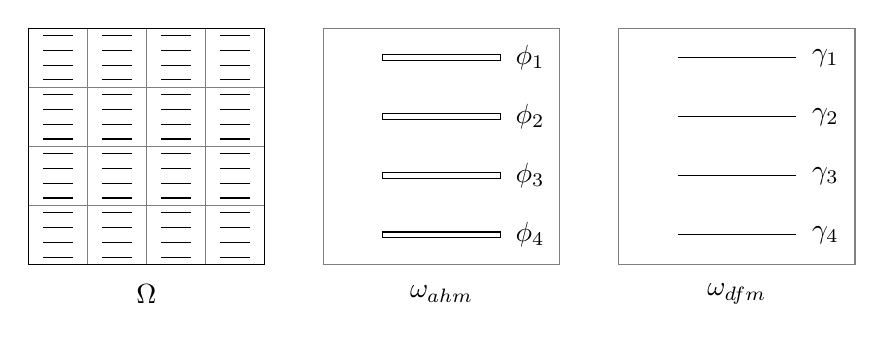
\begin{tikzpicture}[scale=0.75]
        \draw[gray] (0, 0) grid (4, 4);
        \draw (0, 0) rectangle (4, 4);
        \node at (2, -0.5) {$\Omega$};
        \foreach \i in {1,...,4} {
            \foreach \j in {1,...,4} {
                \foreach \k in {1,...,4} {
                    \draw (\i-0.75, \j-\k/4+1/8)--(\i-0.25, \j-\k/4+1/8);
                }
            }
        }
        \draw[gray] (5, 0) rectangle (9, 4);
        \node at (7, -0.5) {$\omega_{ahm}$};
        \foreach \k in {1,...,4} {
            \draw (6, \k-0.55) rectangle (8, \k-0.45);
            \node at (8.5, 4.5-\k) {$\phi_\k$};
        }
        \draw[gray] (10, 0) rectangle (14, 4);
        \node at (12, -0.5) {$\omega_{dfm}$};
        \foreach \k in {1,...,4} {
            \draw (11, \k-0.5) -- (13, \k-0.5);
            \node at (13.5, 4.5-\k) {$\gamma_\k$};
        }
    \end{tikzpicture}
    \caption{Problem domain $\Omega$, subdomain $\omega_{ahm}$ for AHM and $\omega_{dfm}$ for DFM}
    \label{fig:domain}
\end{figure}

\begin{figure}[H]
    \centering
    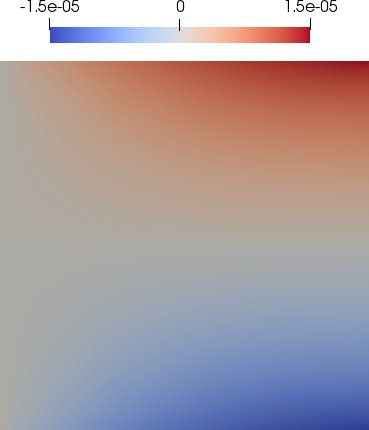
\includegraphics[width=0.2\linewidth]{data/ux.png} \hspace{1em}
    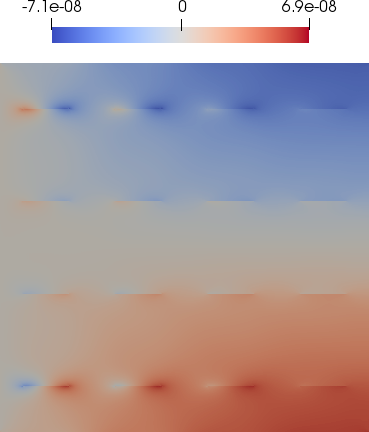
\includegraphics[width=0.2\linewidth]{data/edx.png} \hspace{1em}
    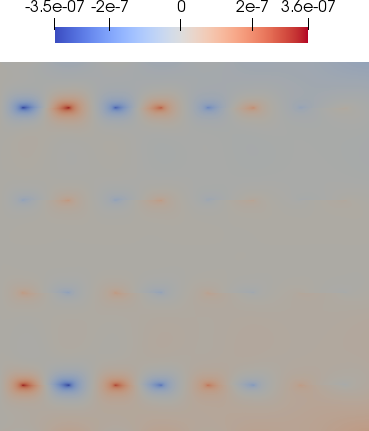
\includegraphics[width=0.2\linewidth]{data/eax.png}\\
    $\hspace{2em} u_1^{fem} \hspace{7em} u_1^{dfm}-u_1^{fem} \hspace{7em} u_1^{ahm}-u_1^{fem}$ \\
    \vspace{1em}
    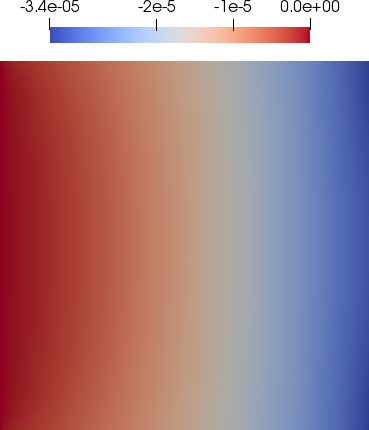
\includegraphics[width=0.2\linewidth]{data/uy.png} \hspace{1em}
    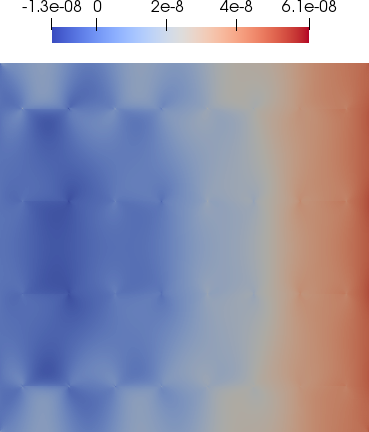
\includegraphics[width=0.2\linewidth]{data/edy.png} \hspace{1em}
    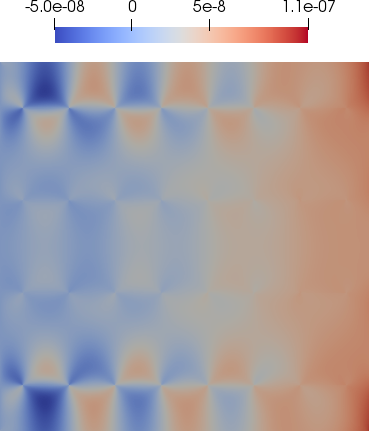
\includegraphics[width=0.2\linewidth]{data/eay.png}\\
    $\hspace{2em} u_2^{fem} \hspace{7em} u_2^{dfm}-u_2^{fem} \hspace{7em} u_2^{ahm}-u_2^{fem}$ \\
    \caption{FEM solution, DFM and AHM errors components}
    \label{fig:solution}
\end{figure}

In our numerical investigation we use the following model parameters:
$E_1 = 2\cdot10^{10}, E_2 = \alpha E_1, \nu_1 = \nu_2 = 0.3, \bm{g} = (0, -10^5),$
where $\alpha$ is the ratio of Young modulus. 
In fig. \ref{fig:solution} we show FEM solution, DFM and AHM errors for parameters: $k = 1, d = 1/1024, \alpha = 32, n = 4, h = 1/2048$.
The error of the DFM solution mostly depends on displacement magnitude and the error of AHM localized near fibers.

Let denote two norms of relative errors by
\[
    \epsilon^{i}_{L_\infty} = \frac{\Vert \bm{u}^{i} - \bm{u}^{fem} \Vert_{L_\infty}}{\Vert \bm{u}^{fem} \Vert_{L_\infty}}, \quad
    \epsilon^{i}_{L_2} = \frac{\Vert \bm{u}^{i} - \bm{u}^{fem} \Vert_{L_2}}{\Vert \bm{u}^{fem} \Vert_{L_2}}, \quad
    i = dfm, ahm, 
\]
where $\bm{u}^{fem}$ is the FEM reference solution, $\bm{u}^{dfm}$ is the DFM solution and $\bm{u}^{ahm}$ is the AHM solution.
We compare DFM and AHM implementations in 5 tests. In each test we vary one of this parameters: $k$, $d$, $\alpha$, $n$, $h$, and all other parameters are fixed.

\begin{figure}[H]
    \centering
    \begin{tikzpicture}[scale=0.95]
        \begin{axis}[
            xmode=log,
            ymode=log,
            log basis x=2,
            log basis y=2,
            xlabel={$k$, number of fibers in $\omega$},
            grid=major,
            legend pos=north west,
            legend columns=2]
            \addplot[mark=square*,solid,red] table[y=edli]{data/k.txt};
            \addplot[mark=square*,solid,blue] table[y=eali]{data/k.txt};
            \addplot[mark=*,dashed,red] table[y=edl2]{data/k.txt};
            \addplot[mark=*,dashed,blue] table[y=eal2]{data/k.txt};
            \addlegendentry{$\epsilon^{dfm}_{L_\infty}$}
            \addlegendentry{$\epsilon^{ahm}_{L_\infty}$}
            \addlegendentry{$\epsilon^{dfm}_{L_2}$}
            \addlegendentry{$\epsilon^{ahm}_{L_2}$}
        \end{axis}
    \end{tikzpicture}
    \hfill
    \begin{tikzpicture}[scale=0.95]
        \begin{axis}[
            xmode=log,
            ymode=log,
            log basis x=2,
            log basis y=2,
            xlabel={$d$, thickness of fibers},
            grid=major,
            legend pos=north west,
            legend columns=2]
            \addplot[mark=square*,solid,red] table[y=edli]{data/d.txt};
            \addplot[mark=square*,solid,blue] table[y=eali]{data/d.txt};
            \addplot[mark=*,dashed,red] table[y=edl2]{data/d.txt};
            \addplot[mark=*,dashed,blue] table[y=eal2]{data/d.txt};
            \addlegendentry{$\epsilon^{dfm}_{L_\infty}$}
            \addlegendentry{$\epsilon^{ahm}_{L_\infty}$}
            \addlegendentry{$\epsilon^{dfm}_{L_2}$}
            \addlegendentry{$\epsilon^{ahm}_{L_2}$}
        \end{axis}
    \end{tikzpicture}
    \caption{Error depending on number and thickness of fibers}
    \label{fig:kd}
\end{figure}

\begin{figure}[H]
    \centering
    \begin{tikzpicture}[scale=0.95]
        \begin{axis}[
            xmode=log,
            ymode=log,
            log basis x=2,
            log basis y=2,
            xlabel={$\alpha$, ratio of Young modulus},
            grid=major,
            legend pos=north west,
            legend columns=2]
            \addplot[mark=square*,solid,red] table[y=edli]{data/f.txt};
            \addplot[mark=square*,solid,blue] table[y=eali]{data/f.txt};
            \addplot[mark=*,dashed,red] table[y=edl2]{data/f.txt};
            \addplot[mark=*,dashed,blue] table[y=eal2]{data/f.txt};
            \addlegendentry{$\epsilon^{dfm}_{L_\infty}$}
            \addlegendentry{$\epsilon^{ahm}_{L_\infty}$}
            \addlegendentry{$\epsilon^{dfm}_{L_2}$}
            \addlegendentry{$\epsilon^{ahm}_{L_2}$}
        \end{axis}
    \end{tikzpicture}
    \hfill
    \begin{tikzpicture}[scale=0.95]
        \begin{axis}[
            xmode=log,
            ymode=log,
            log basis x=2,
            log basis y=2,
            xlabel={$n$, number of subdomains in one direction},
            grid=major,
            legend pos=north east,
            legend columns=2]
            \addplot[mark=square*,solid,red] table[y=edli]{data/n.txt};
            \addplot[mark=square*,solid,blue] table[y=eali]{data/n.txt};
            \addplot[mark=*,dashed,red] table[y=edl2]{data/n.txt};
            \addplot[mark=*,dashed,blue] table[y=eal2]{data/n.txt};
            \addlegendentry{$\epsilon^{dfm}_{L_\infty}$}
            \addlegendentry{$\epsilon^{ahm}_{L_\infty}$}
            \addlegendentry{$\epsilon^{dfm}_{L_2}$}
            \addlegendentry{$\epsilon^{ahm}_{L_2}$}
        \end{axis}
    \end{tikzpicture}
    \caption{Error depending on ration of Young modulus and number of subdomains}
    \label{fig:fn}
\end{figure}

In fig. \ref{fig:kd} we show comparison of relative errors for different number $k$ and thickness $d$ of fibers. For these calculations we fix the next parameters: $n = 4, d = 1/1024, \alpha = 32, h = 1/2048$.
As we can see that both relative errors of DFM are almost the same. And the AHM $L_\infty$ norm of error much higher than $L_2$ due to localization of error near fibers. Both methods show that the relative errors increase with a number of fibers. For all cases $k$, the error $L_2$ norms are similar and differs less than 2 times. And DFM error $L_\infty$ norm is better more than 2 times comparing to AHM.
DFM solution is more sensitive to the thickness of fibers $d$ and the relative error grows faster than AHM error. But for fibers with a small thickness, i.e. with a high ratio of length and thickness, DFM gives more precise solution than AHM.

In next two tests we investigate dependence on $\alpha$ ration of Young modulus and $n$ number of subdomain. Calculated relative errros are plotted in fig. \ref{fig:fn}. For simulations with $\alpha$ variation, we use the following parameters: $n = 4, d = 1/1024, k = 1, h = 1/2048$ and for $n$ variation: $d = 1/1024, k = 1, h = 1/(128\, n)$. DFM solution shows better accuracy for high $\alpha$ ratio of Young modulus and the error is almost constant for different $\alpha$. AHM errror increses with $\alpha$. But as expected AHM error decreases on increasing $n$ number of subdomains. For large $n$ AHM accuracy better than DFM and DFM error increase linearly with number of subdomains. 

\begin{figure}[H]
    \centering
    \begin{tikzpicture}[scale=1]
        \begin{axis}[
            xmode=log,
            ymode=log,
            log basis x=2,
            log basis y=2,
            xlabel={$h$, grid step},
            grid=major,
            legend style={at={(0.03,0.57)},anchor=north west},
            legend columns=2]
            \addplot[mark=square*,solid,red] table[y=edli]{data/h.txt};
            \addplot[mark=square*,solid,blue] table[y=eali]{data/h.txt};
            \addplot[mark=*,dashed,red] table[y=edl2]{data/h.txt};
            \addplot[mark=*,dashed,blue] table[y=eal2]{data/h.txt};
            \addlegendentry{$\epsilon^{dfm}_{L_\infty}$}
            \addlegendentry{$\epsilon^{ahm}_{L_\infty}$}
            \addlegendentry{$\epsilon^{dfm}_{L_2}$}
            \addlegendentry{$\epsilon^{ahm}_{L_2}$}
        \end{axis}
    \end{tikzpicture}
    \caption{Error depending on grid step}
    \label{fig:h}
\end{figure}

Last test is made to compare errors depending on $h$ grid step, see fig. \ref{fig:h}. To neglect FEM error we solve the reference solution on the finest grid with step $h=1/2048$. Also due to variation of grid step, we choose large thickness of fibers $d=1/64$, i.e length and thickness ratio $l/d=8$ and DFM error is larger than AHM error. Other parameters: $n=4, k=1, \alpha=32$.
For fine grids, the errors are close to methods approximation errors and are almost constant. AHM error increases for coarse grids what corresponds to theory. But DFM error decreases for coarse grids due to opposite signs of FEM (in DFM) and DFM errors, which neglect each other.


\section{Conclusion}
We numerically investigated two approaches of deformation modeling of fiber-reinforced materials. DFM comparing to AHM showed better accuracy for a large ration of Young modulus between main material and fibers. Also DFM more convenient for thick fibers, which have a large ration of length and thickness. AHM solution is better for domains containing a large number of equal subdomains. And one of the most important advantages of DFM is using more coarse meshes, where fibers are represented as lines, which reduces degrees of freedom.

\section*{References}
\begin{thebibliography}{}

\bibitem{smarzewski2019influence}
Smarzewski, P.:
Influence of basalt-polypropylene fibres on fracture properties of high performance concrete.
Composite Structures 209, 23-33 (2019)

\bibitem{savspv2018}
Sivtseva, A.V.,  Sivtsev, P.V.:
Numerical Simulation of Deformations of Basalt Roving.
International Conference on Finite Difference Methods, 501--508 (2018).

\bibitem{Kolesov}
Kolesov A. E. et al.:
Numerical Analysis of Reinforced Concrete Deep Beams.
International Conference on Numerical Analysis and Its Applications. – Springer, Cham, 414-421 (2016).

\bibitem{Zakharov}
Zakharov, P.E., Sivtsev, P.V.:
Numerical calculation of the effective coefficient in the problem of linear elasticity of a composite material. 
Mathematical notes of NEFU 24.2, 75-84 (2017).

\bibitem{stepanov2018generalized}
Stepanov, S.P., Vasilyeva, M.V., Vasil’ev, V.I.:
Generalized multiscale discontinuous Galerkin method for solving the heat problem with phase change.
Journal of Computational and Applied Mathematics 340, 645-652 (2018).

\bibitem{DFM}
Vasil’ev V. I. et al.: 
Numerical solution of a fluid filtration problem in a fractured medium by using the domain decomposition method. 
Journal of Applied and Industrial Mathematics 12(4), 785-796 (2018).

\bibitem{DFM2}
Akkutlu I. Y. et al.: 
Multiscale model reduction for shale gas transport in a coupled discrete fracture and dual-continuum porous media. 
Journal of Natural Gas Science and Engineering 48, 65-76 (2017).

\bibitem{fenics2012} 
Logg, A., Mardal, K.A., Wells, G.N.:
Automated solution of differential equations by the finite element method.
Springer (2012).

\bibitem{pinho-da-crus2009asymptotic}
Pinho-da-Cruz J., Oliveira J. A., Teixeira-Dias F. Asymptotic homogenisation in linear elasticity. Part I: Mathematical formulation and finite element modelling. Computational Materials Science 45(4), 1073-1080 (2009)

\bibitem{oliveira2009asymptotic}
Oliveira J. A., Pinho-da-Cruz J., Teixeira-Dias F. Asymptotic homogenisation in linear elasticity. Part II: Finite element procedures and multiscale applications. Computational Materials Science 45(4), 1081-1096 (2009)

\bibitem{pellegrino1999numerical}
Pellegrino C., Galvanetto U., Schrefler B. A. Numerical homogenization of periodic composite materials with non‐linear material components. International Journal for Numerical Methods in Engineering 46(10), 1609-1637 (1999)
    
\bibitem{yuan2008toward}
Yuan Z., Fish J. Toward realization of computational homogenization in practice. International Journal for Numerical Methods in Engineering 73(3), 361-380 (2008)


\end{thebibliography}

\end{document}
